
\documentclass[
	12pt, % Default font size, values between 10pt-12pt are allowed
	%letterpaper, % Uncomment for US letter paper size
	%spanish, % Uncomment for Spanish
]{fphw}

\usepackage{graphicx}
\usepackage{amsthm,amsmath,amssymb}
\usepackage{amsmath,amsfonts,amssymb,amsthm}
\usepackage{physics}
\usepackage{mathtools}
%\usepackage{physics}
\usepackage{algpseudocode}
\usepackage{covington}
\usepackage{algorithm}
\usepackage{setspace}
\usepackage[T1]{fontenc}
\usepackage[labelformat=empty]{caption}
\usepackage{enumerate} % To modify the enumerate environment
%\usepackage{xepersian}
\DeclarePairedDelimiter\ceil{\lceil}{\rceil}
\DeclarePairedDelimiter\floor{\lfloor}{\rfloor}
\DeclarePairedDelimiterX{\inner}[2]{\langle}{\rangle}{#1, #2}

\theoremstyle{plain}
\newtheorem{assumption}{Assumption}


\let\origtheassumption\theassumption 


\thispagestyle{empty}
%\settextfont{Calibri}

\setlength\parindent{0pt}
\title{Differential geometry HomeWork2}
\author{}
\begin{document}
%\maketitle
	%	\doublespacing
\begin{center}
	\noindent\text{ In The Name Of God}\\[5pt]
\end{center}
\begin{center}
    \noindent\text{Mohammad Hossein Heidari Beni (9525983)}\\[5pt]
    \noindent\text{Mohammad Hasan Motamedi (9533713)}\\[5pt]
    \noindent\text{Yousef Javaherian (9525203)}\\[5pt]
    \noindent\text{Mohammad Matin Mazaheri (9533768)}\\[5pt]

\end{center}
‌‌‌‌\begin{center}
    \noindent\text{Exercise 1.2 the Shifrin's book question 4 to 27}\\[5pt]
\end{center}
%\begin{latin}
\section*{Problem 4}
\begin{problem}
     Prove that the curvature of the plane curve \(y=f(x)\) is given by \(\kappa=\frac{\abs{f^{''}}}{(1+f^{'^{2}})^(3/2)}\)
\end{problem}
\subsection*{Answer}
assumption $\alpha$ is the parametrization curve of \(y=f(x)\), then we can write :\\
\begin{align*}
     \alpha(t) &= (t,f(t))\\
     \alpha'(t) &= (1,f'(t))\\
     \alpha''(t) &= (0,f''(t))\\
     \implies\kappa &= \frac{\parallel{\alpha' \times \alpha''}\parallel}{\parallel\alpha'\parallel^3}=\frac{\abs{f^{''}}}{(1+f^{'^{2}})^(3/2)}\
\end{align*}
\section*{Problem 5}
\begin{problem}
     Use Proposition 2.2(page 14) and the second parametrization of the tractrix given in Example 2 of Section 1(page 5) to
      recompute the curvature.
\end{problem}
\subsection*{Answer}
     if $\alpha$ is the second parametrization of the tractrix and $\kappa = \frac{\parallel{\alpha' \times \alpha''}\parallel}{\parallel\alpha'\parallel^3}$\\
     and $s = \sech(t),r = \tanh(t)$ then:\\
     \begin{align*}
          \alpha(t) &= (t - \tanh(t),\sech(t))\\
          &\implies\alpha'(t) = (1 - s^2,-sr) = (r^2,-sr)\\
          &\implies\alpha''(t) = (2rs^2,-s^3 + r^2s)\\
          &\implies\kappa = \frac{\abs{r^2s^3 + r^4s}}{r^3} = \frac{s^3 + r^2s}{r} = \frac{s^3 + (1-s^2)s}{r} = \frac{s}{r}\\
          (s = \sech(t),r = \tanh(t))&\implies\kappa = \frac{1}{\sinh(t)}
     \end{align*}
     verifing the result by setting $e^t = \tan(\theta/2)$:
     \begin{align*}
          \kappa &= \frac{1}{\sinh(t)} = \frac{2}{e^t - e^(-t)} = \frac{2e^t}{e^(2t) - 1} = \frac{2\tan(\theta/2)}{tan(\theta/2)^2 - 1} = \frac{2\sin(\theta/2)\cos(\theta/2)}{\sin(\theta/2)^2 - \cos(\theta/2)^2}\\
          \implies\kappa &=  \frac{\sin(\theta)}{-\cos(\theta)} = -\tan(\theta)\\
     \end{align*}
     is same as the result of example(2)

\section*{Problem 6}
\begin{problem}
     By differentiating the equation \(B = T \times N\),derive the equation \(B^{'} = -\iota N\).
\end{problem}

\subsection*{Answer}
by derived from B we have:
\begin{align*}
     B' &= T' \times N + T \times N' = kN \times N + T \times (-kT + \iota B) = \iota T \times B = -\iota N\\
     \implies B' &= -\iota N\\
\end{align*}
\section*{Problem 7}
\begin{problem}
     Suppose \(\alpha\) is an arclength-parametrized space curve with the property that $||\alpha(s)||<||\alpha(s0)|| = R$ for
all s sufficiently close to s0. Prove that \(\kappa(s0) >= 1/R\). (Hint: Consider the function $f (s) = ||\alpha(s)||^{2}$.
What do you know about \(f^{''} (s0)\)
\end{problem}
\subsection*{Answer}
Suppose \(\alpha\) is an arclength-parameterized space curve with the property that $||\alpha(s)||<||\alpha(s0)|| = R$ for
all s sufficiently close to s0. Prove that \(\kappa(s0) >= 1/R\). (Hint: Consider the function $f (s) = ||\alpha(s)||^{2}$.
What do you know about \(f^{''} (s0)\)
\subsection*{Answer}

\begin{align*}
    \forall s \in N_\epsilon(s_0) : ||\alpha(s)||^2 \leq ||\alpha(s_0)||^2
\end{align*}
    therefore  $f(s)=||\alpha(s)||^2$  has negative curvature, that is
\begin{align*}
    f''(s) \leq 0
\end{align*}
on the other hand
\begin{align*}
     f(s) = ||\alpha||^2 \implies f'(s)=2\alpha(s)\cdot \alpha'(s) \implies 
     f''(s)=2||\alpha'(s)||^2 + 2\alpha(s)\cdot \alpha''(S) \\
     \implies f''(S)=2\left( 1+k\alpha(s)\cdot N(s)\right)\\
\end{align*}
     hence
\begin{align*}
     1+k(s_0)\alpha(s_0)\cdot N(s_0) \implies 1+k(s_0)R\cos(\theta) \leq 0
\end{align*}
    where $\theta$ is angle between $\alpha$ and $N$ at $s_0$
\begin{align*}
     k(s_0)R\cos(\theta)\leq -1 \implies k(s_0)R\left[-\cos(\theta)\right] \geq 1 \implies k(s_0)R \geq 1
\end{align*}
We can also justify above inequality intuitively by noting that if $k(s_0) = \frac{1}{R}$ \\
then $\alpha$ would behaved like a circle around $s_0$ meaning that points near $s_0$ all would have had the same absolute value as $s_0$ but we know that $||\alpha(s)|| \leq ||\alpha(s_0)||$ hence curvature must be greater than a circle.


\section*{Problem 8}
\begin{problem}
     Let $\alpha$ be a regular (arclength-parametrized) curve with nonzero curvature. The normal line to $\alpha$ at $\alpha(s)$
is the line through $\alpha(s)$ with direction vector N(s) Suppose all the normal lines to $\alpha$ pass through a fixed point. What can you say about the curve?
\end{problem}
\subsection*{Answer}
\begin{align*}
     \alpha(s) - P = \lambda(s)N(s) \implies T(s)=\lambda'(s)N(s) + \lambda(s)\left( -k(s)T(s) + \tau(s)B(s) \right)
 \end{align*}
 \begin{align*}
 \lambda^{'}(s)=0\\
 1+\lambda(s)k(s)=0\\
 \lambda(s)\tau(s)=0
 \end{align*}
     $\implies$
 \begin{align*}
 \tau=0 \implies \alpha  lies on a plane \\
 k is a non-zero constant.
 \end{align*}  
now only planer curve with constant non-zero curvature is a circle (part of a circle) so $\alpha$ is a circle.
 

\section*{Problem 9}
\begin{problem}
     Prove that if all the normal planes of a curve pass through a particular point, then the curve lies on a sphere. (Hint: Apply Lemma 2.1.)
\end{problem}
\subsection*{Answer}
\subsubsection*{a}
\begin{align*}
    \left( \alpha - P \right)\cdot T = 0 \implies \left( \alpha - P\right)\left( \alpha' - P'\right) = 0\\
    \implies ||\alpha - P|| = constant.
\end{align*}
Hence $\alpha$ is on a sphere.

\subsubsection*{b}
\begin{align*}
    \left( \alpha - P \right)\cdot B = 0 \implies \alpha'\cdot B + \left( \alpha - P \right) \left( -\tau\nu N\right)=0
    \tau \left( \alpha - P \right)\cdot N = 0\\
    \implies \tau\left( \alpha - P \right)\cdot N + \tau \alpha'\cdot N + z\left(\alpha-P\right)\nu \cdot \left(-kT + \tau B) = 0\right)
\end{align*}
Now note that projection of $\alpha - P$ on all of $T, N, B$ can not be zero at same time. therefore $k\tau=0 \implies \tau=0$. Hence $\alpha$ is planar.

\section*{Problem 10}
\begin{problem}
     Prove that if $\kappa = \kappa_{0}$ and $\tau = \tau_{0}$ are nonzero constants, then the curve is a (right) circular helix.\\
     (Hint: Start by solving for N. The only solutions of the differential equation $y^{''} + k^2 y = 0$ are $y = c1 cos(kt) + c2 sin(kt)$.)\\
     Remark. It is an amusing exercise to give a and b (in our formula for the circular helix) in terms
of $\kappa_{0}$ and $\tau_{0}$.
\end{problem}
\subsection*{Answer}
Let us assume that the curve $\alpha$ is arclength-parameterized
\begin{align*}
& T' = kN\\
& N' = -kT + \tau B \implies N'' = -k^{2}N - \tau^{2}N = -\lambda^{2}N\\
& B' = -\tau N \implies N = c_1 \cos(\lambda s) + c_2 \sin(\lambda s)\\
& \implies T = c_3 + c_1\cos(\lambda s) + c_2\sin(\lambda s)\\
& \implies \alpha = c_4 + c_3 s + c_1\cos(\lambda s) + c_2\sin(\lambda s)
\end{align*}
Where $c_1 - c_4$ are arbitrary vector constants such that $||a'||=1$.
If we want to represent a circular helix we need to set :
\begin{align*}
&c_4=0 &c_3 = c_3 \lambda \hat{z} \\
&c_2 = c_1\hat{y} & c_1 = c_1 \hat{x}
\end{align*}
Then 
\begin{align*}
&\alpha=[c_1\cos(\lambda s), c_1\sin(\lambda s), c_3\lambda s]\\
&\implies \alpha' = [-\lambda c_1\sin(\lambda s), \lambda c_1\cos(\lambda s), c_3\lambda]\\
&\implies ||\alpha'||^2 = c_{3}^2\lambda + c_{1}^2\lambda\\
&\implies \lambda = \frac{1}{\sqrt{c_{1}^2 + c_{3}^2}}\\
&\implies \alpha = [c_1\cos{\frac{s}{\sqrt{c_{1}^2 + c_{3}^2}}}, c_1\sin{\frac{s}{\sqrt{c_{1}^2 + c_{2}^2}}}, {\frac{c_3 s}{\sqrt{c_{1}^2 + c_{3}^2}}}]
\end{align*}

\section*{Problem 11}
\begin{problem}
     Proceed as in the derivation of Proposition 2.2 to show that\\
     \begin{center}
          $\tau = \frac{\inner{\alpha^{'}}{\alpha^{''} \times \alpha^{'''}}}{||(\alpha^{'} \times \alpha^{''})||^{2}}$
     \end{center}
\end{problem}
\subsection*{Answer}
\begin{align*}
&\alpha'=\nu T \\
&\alpha''=\nu'T+\nu^2 kN\\
&\alpha^3 = \nu^4T+3\nu\nu'kN+\nu^2k'N+\nu^3k(-kT+\tau B)\\
&\implies\alpha'\cdot (\alpha''\times\alpha''')=\alpha'\cdot[\nu^2kN\times((3\nu\nu'k+\nu^2k')N+\nu^3k\tau B]=\alpha'\cdot\nu^2k\nu^3k\tau N\times B = \nu^6k^2\tau\\
&||\alpha'\times\alpha''||^2 = ||\nu^3kB||^2=(\nu^3k)^2=\nu^6k^2\\
&\implies\frac{\alpha'\cdot(\alpha''\times\alpha''')}{||\alpha'\times\alpha''||^2}=\frac{\nu^6k^2\tau}{\nu^6k^2}=\tau
\end{align*}

\section*{Problem 12}
\begin{problem}
     Let $\alpha$ be a $c^4$ arclength-parametrized curve with $\kappa \neq 0$. Prove that $\alpha$ is a generalized helix if and only
if $\inner{\alpha^{''}}{\alpha^{'''} \times \alpha^{(iv)}}= 0$. (Here $\alpha^{(iv)}$ denotes the fourth derivative of $\alpha$)
\end{problem}
\subsection*{Answer}
\setcounter{assumption}{0}
\setcounter{equation}{0}
at first, we are trying to simplified the equation in the question using Frenet equation :
\begin{align}
     \inner{\alpha^{''}}{\alpha^{'''}\times\alpha^{iv}} & = 0 \\
     \inner{kN}{(k^{'}N+kN^{'})\times(k^{''}N+2k^{'}N^{'}+kN^{''})} & = 0 \\
     \inner{kN}{((k^{'}N\times 2k^{'}N^{'})+(k^{'}N\times kN^{''})+(kN^{'}\times k^{''}N)+(kN^{'}\times kN^{''}))} & = 0 \\
     \inner{kN}{(kN^{'} \times kN^{''})} & = 0
\end{align}
now, we should solve the question for this new equation obtained above :
\begin{enumerate}[(\itshape a\normalfont)]
     \item 
     \begin{assumption}-$simplified-question-equation$\label{as:1}
          $\inner{kN}{(kN^{'} \times kN^{''})} = 0$
     \end{assumption}
     from the above assumption we can conclude that all the $N,N^{'},N^{''}$ are in the same plane with the normal $A = \frac{N' \times N}{||N'\times N||}$
     . So $A(s)$ is orthogonal to all of $N,N^{'},N^{''}$ for each $s$. So $A(s)$ , $N(s)$ and $N^{'}(s)$ are a basis for $R^{3}$. now, we want to write $A^{'}(s)$(a vector in $R^{3}$) in terms of $A(s)$ , $N(s)$ and $N^{'}(s)$:
     \begin{align}
         \inner{{N}}{A} & = 0 \\
         (\inner{N}{A})^{'} & = 0 \\
         (\inner{N^{'}}{A})+(\inner{N}{A^{'}}) & = 0 \\
         (\inner{N^{'}}{A}) & = 0 \\
         (\inner{N}{A^{'}}) & = 0
     \end{align}
     Equation 9 is concluded from the definition of A as normal vector for the plane containing $N'$ and according to equation 8 and 9, we can conclude the equation 10. In the same way, We have 
     \begin{align}
          \inner{{N^{'}}}{A} & = 0 \\
          (\inner{N^{'}}{A})^{'} & = 0 \\
          (\inner{N^{''}}{A})+(\inner{N^{'}}{A^{'}}) & = 0 \\
          (\inner{N^{''}}{A}) & = 0 \\
          (\inner{N^{'}}{A^{'}}) & = 0
      \end{align}
      according to the fact that A(s) is unit vector for each $s$ We can write :
      \begin{align}
          \inner{A}{A} & = 1\\
          (\inner{A}{A})^{'} & = 0 \\
          (\inner{A^{'}}{A}) & = 0  
      \end{align}
      According to the equation 10,15 and 18 . $A^{'}(s) = 0*N(s)+0*N^{'}(s)+0*A(s)$ for each s. So $A^{'}(s)=0$ and we can say that $A(s)=const$ and write that:
      \begin{align}
          \inner{N}{A} & = 0\\
          (\inner{T^{'}}{A}) & = 0 \\
          (\inner{T}{A}) & = c 
      \end{align}  
      Because $k \neq 0 $, we can conclude 20 from 19. According to the last equation $\alpha$ and the fact that $k \neq 0  $ is generalized helix in $R^{3}$.
     \item 
     \begin{assumption}
          $\alpha$ is generalized helix
     \end{assumption} 
     From the above assumption, we can say that there is fixed unit vector $A$ with the following features:
     \begin{align}
          \inner{T}{A} & = const\\
          (\inner{T^{'}}{A}) & = 0 \\
          (\inner{N}{A}) & = 0 \\
          (\inner{N^{'}}{A}) & = 0 \\
          (\inner{N^{'}}{A}) & = 0
      \end{align}
      Because $k \neq 0$ we can conclude equation 23 from 22. As we know at least there is an orthogonal base set for $R^{3}$ including vector $A$. According to the above equations, $N$,$N^{'}$ and $N^{''}$ is written in term of two other base vectors in orthogonal base vector set including A for $R^{3}$. So they lie on the plane spaned with orthogonal vectors in the base set except vector A. So we have:
      \begin{align}
          \inner{kN}{(kN^{'} \times kN^{''})} & = 0 \\
          \inner{\alpha^{''}}{\alpha^{'''}\times\alpha^{iv}} & = 0 
     \end{align}
      Equation 26 is concluded from equation 25 according to the equations 1 to 4.
\end{enumerate}

\section*{Problem 13}
\begin{problem}
     Suppose $\kappa\tau \neq 0$ at $P$. Of all the planes containing the tangent line to $\alpha$ at P, show that $\alpha$ lies locally on both sides only of the osculating plane.
\end{problem}
\subsection*{Answer}
\subsection*{Answer}
\setcounter{assumption}{0}
\setcounter{equation}{0}
As N and B is orthogonal to T at P, we can write all possible unit normal vectors for the planes containing the tangent line of $\alpha$ at P 
in terms of N and B. So we have:
\begin{align}
     A & = \sin(\theta)N_{p}+\cos(\theta)B_{p} \\ 
\end{align}
To check that the plane $\alpha$ is locally on both sides of which of the above plane we should use the following equation for all point which is locally near the point P on curve $\alpha$ to compute
the inner product of each vector started from the (0,0) to each of these points with all possible the normal vectors of the above plane.
\begin{equation}
     \alpha(s)-\alpha(s_{p}) = ((s-s_{p})-\frac{\kappa_{p}(s-s_p)^{3}}{6}) T_p + (\kappa_{p}/2(s-s_{p})^{2}+\frac{\kappa^{'}_{p}(s-s_p)^{3}}{6}) N_p + (\frac{\kappa_{p}\tau_{p}(s-s_p)^{3}}{6}) B_p\\ 
\end{equation}
To compute the inner product $\inner{\alpha(s)-\alpha(s_{p})}{A}$, We write:
\begin{equation}
     \inner{\alpha(s)-\alpha(s_{p})}{A} = (s-s_p)^{2}(\sin(\theta) \kappa_{p}/2  + \sin(\theta)(s-s_{p})\kappa^{'}_{p}/6  + \cos\theta (s-s_{p})(\kappa_{p}\tau_p)/6) 
\end{equation}
According to the above equation, $s_{p}$ is the second root of the inner product  except when $\theta=0$. If $\theta\neq0$, the sign of the inner product don't change locally on range $(s_{p}-\epsilon,s_{p}+\epsilon)$
and this means the points near P on $\alpha$ remain on one side of the plane with normal vector $\sin(\theta)N+\cos(\theta)B$. But only when $\theta=0$ the sign of inner product change in range $((s_{p}-\epsilon,s_{p}+\epsilon))$ by passing through $s_p$ and this means that $\alpha$
don't remain the one side near point P. So $\alpha$ lies locally at P on both side of the plane with the normal vector $\sin(0)N_{p}+\cos(0)B_{p}=B_{p}$. So the only plane with the normal vector $B_p$ is the osculating plane at P which is spanned with $T_{p}$ and $N_{p}$.

\section*{Problem 14}
\begin{problem}
     Let $\alpha$ be a regular curve with $\tau \neq 0$ at P. Prove that the planar curve obtained by projecting $\alpha$ into its
osculating plane at P has the same curvature at P as $\alpha$.
\end{problem}
\subsection*{Answer}
assuming $||\alpha'||=1$ we can write $P=\alpha(t_0)$
\begin{align*}
&\beta = \alpha - [(\alpha - P)\cdot B(t_0)]B(t_0) \\
&\beta' = \alpha' - [\alpha'\cdot B(t_0)]B(t_0) \implies \beta'(t_0)=\alpha'(t_0) \\
&\beta'' = \alpha'' - [\alpha''\cdot B(t_0)]B(t_0) \implies \beta''(t_0)=\alpha''(t_0) \\
&k_\beta(t_0) = \frac{||\beta' \times \beta''||}{||\beta'||^3}|_{t=t_0} = \frac{||\alpha' \times \alpha''||}{||\alpha'||^3}|_{t=t_0} = k_\alpha (t_0)
\end{align*}


\section*{Problem 15}
\begin{problem}
     A closed, planar curve $C$ is said to have constant breadth $\mu$ if the distance between parallel tangent
lines to C is always . (No, C needn’t be a circle. See Figure 2.5.) Assume for the rest of this problem
that the curve is arclength parametrized by a C2 function $\alpha:[0,L]-> R^{2}$ with $\tau \neq 0$. To say C is closed
means $\alpha(0) = \alpha(L)$ and the derivatives match as well.
\begin{enumerate}[(\itshape a\normalfont)] % Sub-questions styled as italic letters
     \item Let’s call two points with parallel tangent lines opposite. Prove that if C has constant breadth
     $\mu$, then the chord joining opposite points is normal to the curve at both points. (Hint: If $\beta(s)$ is
     opposite $\alpha(s)$, then $\beta(s) = \alpha(s) + \lambda(s)T(s)+ \mu N(s)$. First explain why the coefficient of N is $\mu$
     then show that $\lambda = 0$.)
     \item Prove that the sum of the reciprocals of the curvature at opposite points is equal to $\mu$. (Warning: If
     $\alpha$ is arclength-parametrized $\beta$ is quite unlikely to be. It might be helpful to introduce the notation
     $T_{\beta}$ and $N_{\beta}$ for the unit tangent vector and principal normal of $\beta$. How are they related to T and
     N?)
\end{enumerate}
\end{problem}
\begin{figure}[!ht]
     \centering
     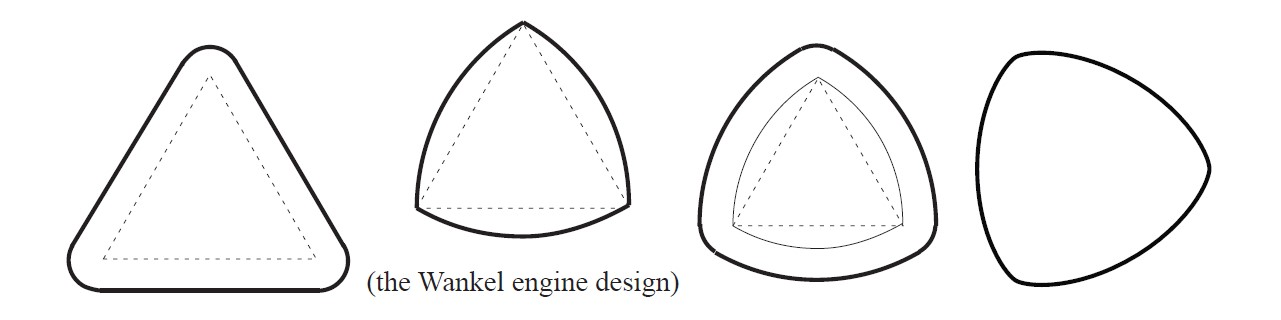
\includegraphics[width=\linewidth, width=14cm, height=6cm]{question_15.jpg}
     \caption{Figure 2.5}
\end{figure}
\subsection*{Answer}

\subsubsection*{a}
\begin{align*}
&[\alpha(t) - \beta(t)]\cdot N = \pm\mu \implies [\alpha'-\beta']\cdot N + [\alpha - \beta]\cdot N'=0\\
&\implies (\alpha-\beta)\cdot (-kT)=0 \xRightarrow{{k\neq0}} (\alpha-\beta)\cdot T_{\alpha}=0\\
&\implies (\alpha-\beta)\cdot T_\beta
\end{align*}
\subsubsection*{b}
\begin{align*}
&\alpha-\beta = \pm\mu N \implies \alpha'-\beta'=\mp\mu kT=\mp \mu k\alpha'\\
&\beta'=(1\pm\mu k)\alpha
\end{align*}
Now because $\alpha$ is a closed curve we expect $\beta'$ to be in opposite direction of $\alpha'$ hence,
\begin{align*}
&1\pm \mu k < 0 \implies 1-\mu k < 0 \implies \mu k > 1 \\
&\beta'=(1-\mu k)\alpha' \implies \beta'' = (1-\mu k)\alpha'' - \mu k'\alpha'
\implies k_\beta \nu_b ^2=||(1-\mu k)\alpha''||\\
&k_b(1-\mu k)^2 = k|1-\mu k| = k(\mu k-1) \implies k_\beta(1-\mu k)=-k\\
&k_\beta + k = kk_\beta \mu \implies \frac{1}{k} + \frac{1}{k_\beta} = \mu
\end{align*}


\section*{Problem 16}
\begin{problem}
     \begin{enumerate}[(\itshape a\normalfont)] % Sub-questions styled as italic letters
          \item  Suppose $\alpha$ is arclength-parametrized. Show that $\beta$ is an involute of $\alpha$ if and only if $\beta(s) =
          \alpha(s)+(c-s)T(s)$ for some constant c (here $T(s) = \alpha(s)$). We will normally refer to the curve $\beta$
          obtained with c = 0 as the involute of $\alpha$. If you were to wrap a string around the curve $\alpha$, starting
          at s = 0, the involute is the path the end of the string follows as you unwrap it, always pulling the
          string taut, as illustrated in the case of a circle in Figure 2.6.
          \item  Show that the involute of a helix is a plane curve.
          \item Show that the involute of a catenary is a tractrix. (Hint: You do not need an arclength parametrization!)
          \item If $\alpha$ is an arclength-parametrized plane curve, prove that the curve $\beta$ given by
          \begin{center}
               $\beta(s) =  \alpha(s) + \frac{N(s)}{\kappa(s)}$
          \end{center}
          is the unique evolute of $\alpha$ lying in the plane of $\alpha$. Prove, moreover, that this curve is regular if
          $\tau^{'} \neq 0$. (Hint: Go back to the original definition.)
     \end{enumerate}
\end{problem}
\begin{figure}[!ht]
     \centering
     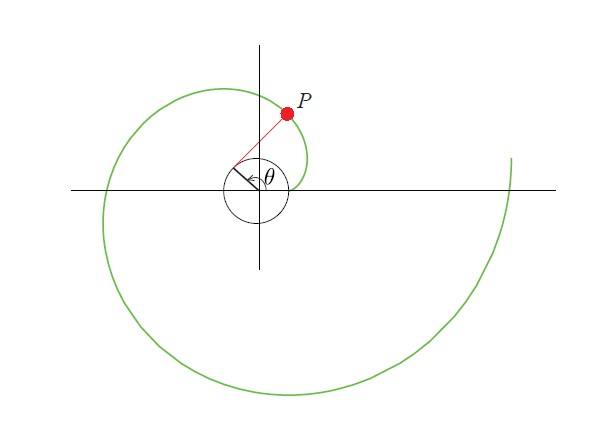
\includegraphics[width=\linewidth, width=14cm, height=6cm]{question_16.jpg}
     \caption{Figure 2.6}
\end{figure}
\subsection*{Answer}

\subsubsection*{a}
\begin{align*}
&\beta = \alpha + (c-t)T_\alpha \implies \beta'=(c-t)\alpha''\implies (\beta-\alpha)||T_\alpha ,   \beta'\bot \alpha'
\end{align*}
Therefore $\beta$ is involute of $\alpha$.
\begin{align*}
&(\beta-\alpha)||T_\alpha \implies \beta=\alpha+\lambda T_\alpha \implies \beta'=\alpha'+\lambda'T_\alpha+\lambda \alpha''\\
&\implies \beta'\cdot \alpha'=a+\lambda'=0 \implies \lambda=c-t \implies \beta=\alpha+(c-t)T_\alpha
\end{align*}
\subsubsection*{b}
\begin{align*}
&\beta=\alpha(s)-sT(s) \implies \beta\cdot \hat{z} = \alpha(s)\cdot\hat{z} - s\alpha'(s)\cdot\hat{z}\\
&\alpha(s)=[a\cos(\frac{s}{c}), a\sin(\frac{s}{c}), \frac{bs}{c}], \alpha'(s)=\frac{1}{c}[-a\sin(\frac{s}{c}), a\cos(\frac{s}{c}), \frac{bs}{c}]\\
&\implies \beta\hat{z} = \frac{bs}{c} - \frac{sb}{c}=0
\end{align*}
Hence $\beta$ lies on the xy-plane.
Please note that we assumed 'helix' is just simple circular helix.

\subsubsection*{c}
In this part we assume the constant $c$ in the definition of a catenary is one.
\begin{align*}
    \alpha(t)=[t, \sinh(t)], \beta'(t)=[\tanh_2(t), -\sech(t), \tanh(t)]
\end{align*}
We need to check that $\alpha'\bot \beta'$ and $\beta - \alpha\bot \beta'$
\begin{align*}
&\alpha'\cdot\beta'=\tanh^2(t) - \tanh^2(t) =0
&-\tanh^3(t)-\sech^3(t)\tanh(t)+\tanh(t)=-\tanh(t)[-1 + \tanh^2(t)+\sech^2(t)]=0
\end{align*}
Now since $\alpha(0)=\beta(0)$ $\beta$ is the involute of $\alpha$.

\subsubsection*{d}
$\beta$ is evolute of $\alpha \iff (\beta-\alpha)\bot T_\beta$,  $T_\alpha\bot T_\beta$.
Now if $\alpha$ is planar and $\beta$ is also on the same plane as $\alpha$
\begin{align*}
&\beta - \alpha||T_\beta \iff \beta - \alpha||T_\alpha
\beta - \alpha\cdot T_\alpha=0 \implies \beta' - \alpha'\cdot T_\alpha+\beta - \alpha\cdot T'_\alpha\\
&\implies (\beta-\alpha)\cdot T'_\alpha=1 \xRightarrow{{\beta - \alpha||T_\alpha}} \beta-\alpha=\lambda N\\
&\lambda N\cdot kN=1 \implies \lambda=\frac{1}{k}\implies \beta=\alpha+\frac{N}{k}\\
&\beta'=\alpha'+\frac{-k^2T-k'N}{k^2}=\frac{-k'N}{k^2}
\end{align*}
Hence $\nu_\beta=\frac{k'}{k^2}$ implies $\beta$ is regular if and only if $k'$ was never zero.


\section*{Problem 17}
\begin{problem}
     Find the involute of the cycloid $\alpha(t) = (t+\sin(t),1 - cos(t) )$, $t \in [-\pi,\pi]$,  using $t = 0$ as your starting
     point. Give a geometric description of your answer.
\end{problem}
\subsection*{Answer}

\begin{align*}
     &\beta=\alpha-S(t)T
     &S(t)=\int_{0}^{t}\nu dt=[t+\sin(t),1-\cos(t)]\\
     &\alpha'=[1+\cos(T), \sin(t)]\implies\nu^2=2(1+\cos(t))=4(\cos^2(t/2))\\
     &\nu=2|\cos(t/2)|\xRightarrow{{\pi/4\leq t/2\leq \pi/2}} \nu=2\cos(t/2),T=\frac{1}{2\cos(t/2)}[1+\cos(t), \sin(t)]\\
     &S(t)=\int_{0}^{t}2\cos(u/2)du=4\sin(u/2)|_{0}^{t}=4\sin(t/2)\\
     &\implies \beta=[t+\sin(t),1-\cos(t)]-\frac{4\sin(t/2)}{2\cos(t/2)}[1+\cos(t), \sin(t)]=[t+\sin(t)-2\sin(t), 1-\cos(t)-4\frac{\sin(\frac{t^2}{2}\cos(t))}{\cos(t/2)}]\\
     &=[t-\sin(t), 1-\cos(t)-4\frac{1-\cos(t)}{2}]=[t-\sin, \cos(t)-1]
\end{align*}
Hence $\beta$ is also a cycloid but is turning CCW and mirrored by the x axis.

\section*{Problem 18}
\begin{problem}
     Suppose $\alpha$ is a generalized helix with axis in direction $A$. Let $\beta$ be the curve obtained by projecting $\alpha$
onto a plane orthogonal to $A$. Prove that the principal normals of $\alpha$ and $\beta$ are parallel at corresponding
points and calculate the curvature of $\beta$ in terms of the curvature of $\alpha$.
\end{problem}
\subsection*{Answer}
lets assume $||\alpha'|| = 1$ and c is a constant we have:\\
\begin{align*}
    &\alpha - \beta = (\alpha - p).AA = [\alpha.A]A - cA\\
    &\implies \beta = \alpha - (\alpha.A)A + cA\\
\end{align*}
so $\implies \beta' = \alpha' - (\alpha'.A)A$ that $\alpha'.A$ is a constant so $\beta'' =\alpha''$ then:\\
\begin{align*}
     &\implies v'_\beta T_\beta + k_\beta v_\beta^2 N_\beta = kN\\
     &\implies v_\beta^2 = \beta'\beta' = [\alpha' - (\alpha'.A)A].[\alpha' - (\alpha'.A)A]\\
     &\implies v_\beta^2 = ||\alpha'||^2 - 2(\alpha'.A)^2 + (\alpha'.A)^2 ||A||^2\\
 \end{align*}
 According to $||A||^2 = 1$ then:\\
 \begin{align*}
     &\implies v_\beta^2 = 1 - (\alpha'.A)^2 = const\\
     &\implies v_\beta' = 0\\
     &\implies k_\beta v_\beta^2 N_\beta = kN
 \end{align*}
 so $k_\beta = \frac{k}{ v_\beta^2} = \frac{k}{ 1 - (A.T)^2}$ and $N_\beta \parallel N$ .



\section*{Problem 19}
\begin{problem}
     Let $\alpha$ be a curve parametrized by arclength with $\kappa$, $\tau \neq 0$.\\
     \begin{enumerate}[(\itshape a\normalfont)] % Sub-questions styled as italic letters
          \item Suppose $\alpha$ lies on the surface of a sphere centered at the origin (i.e., $||\alpha(s)|| = const$ for all $s$).
          Prove that
          \begin{center}
               $\frac{\tau}{\kappa} + (\frac{1}{\tau}(\frac{1}{\kappa})^{'})^{'} = 0$
          \end{center} 
          (Hint: Write $\alpha = \lambda T + \mu N + \vartheta B$ for some functions $\lambda$, $\mu$ and $\vartheta$, differentiate, and use the fact
           that ${T;N;B}$ is a basis for $R^{3}$.)    
          \item Prove the converse: If $\alpha$satisfies the differential equation (*), then $\alpha$ lies on the surface of some
          sphere. (Hint: Using the values of $\lambda$,$\mu$ and $\vartheta$ you obtained in part a, show that $\alpha - (\lambda T+ \mu N + \vartheta B)$
          is a constant vector, the candidate for the center of the sphere. If the nature of this argument puzzles
          you, review the latter part of the proof of Proposition 2.4.)
     \end{enumerate}

\end{problem}
\subsection*{Answer}
\begin{enumerate}[(\itshape a\normalfont)]
     \item According to $||\alpha'||$ is constant then:\\   \\ $\alpha.\alpha' = 0\\  \\ \implies 1 + \alpha.kN =0$\\  \\ $\implies \alpha.N = \frac{-1}{k}$\\  \\$\implies \alpha'N + \alpha'.N + \alpha.(-kT + \tau B) = \frac{1}{k}$\\  
       \\$\implies \alpha.B = \frac{1}{k^2 \tau}$\\  \\$(\alpha'.N)\implies \alpha = (0)T + \frac{-1}{k}N + \frac{1}{k^2 \tau}B$\\  \\$\implies \alpha' = T + (\frac{\tau}{k} + (\frac{1}{k^2 \tau})')B$\\  
         \\$\implies \frac{\tau}{k} + (\frac{1}{\tau}(\frac{1}{k})')' = 0$\\
     \item According to (a) then:\\  \\$\alpha' =  T + (\frac{\tau}{k} + (\frac{1}{k^2 \tau})')B$\\
       \\$\implies \alpha = \frac{-N}{k} + (\frac{1}{k^2 \tau})')B + p$(p is a constant vector)\\
       \\$\implies \alpha - p \bot (\alpha - p)'$\\  \\and in end:\\  \\$||\alpha - p|| =$ constant\\
\end{enumerate}

\section*{Problem 20}
\begin{problem}
     Two distinct parametrized curves $\alpha$ and $\beta$ are called Bertrand mates if for each t , the normal line to $\alpha$
     at $@\alpha(t)$  equals the normal line to $\beta$ at $\beta(t)$. An example is pictured in Figure 2.7. Suppose $\alpha$ and $\beta$ are Bertrand mates.
     \begin{enumerate}[(\itshape a\normalfont)] % Sub-questions styled as italic letters
          \item If $\alpha$ is arclength-parametrized, show that $\beta(s)  = \alpha(s) + r(s)N(S)$ and r(s) = const. Thus,
          corresponding points of $\alpha$ and $\beta$ are a constant distance apart. 
          \item Show that, moreover, the angle between the tangent vectors to $\alpha$ and $\beta$ at corresponding points
          is constant. (Hint: If $T_{\alpha}$ and $T_{\beta}$ are the unit tangent vectors to $\alpha$ and $\beta$ respectively, consider
          $T_{\alpha}aT_{\beta}$.)
          \item Suppose $\alpha$ is arclength-parametrized and $\kappa\tau \neq 0$. Show that $\alpha$ has a Bertrand mate $\beta$ if and only if
          there are constants r and c so that $r\tau + c\kappa = 1$. (Hint for $==>$): Interpret the result of part b using
          your formula for $\beta^{'}$ from part a.)
          \item Given $\alpha$, prove that if there is more than one curve $\beta$ so that $\alpha$and $\beta$ are Bertrand mates, then there
          are infinitely many such curves $\beta$ and this occurs if and only if $\alpha$is a circular helix.
     \end{enumerate}
\end{problem}
\begin{figure}[htbp]
     \centering
     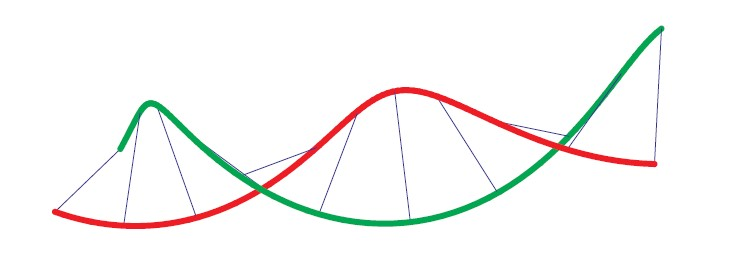
\includegraphics[width=\linewidth, width=14cm, height=6cm]{question_20.jpg}
     \caption{<caption>}
     \label{<label>}
\end{figure}
\subsection*{Answer}
\begin{enumerate}[(\itshape a\normalfont)]
     \item According to problem we have $\beta - \alpha = rN_\alpha , (\beta - \alpha).(\beta' - \alpha') = 0$ so:\\
       \\$||\beta - \alpha|| = r =$ constant\\  \\$\implies \beta(s) = \alpha(s) + rN(s)$ (r is constant)\\
     \item According to problem we have:\\  \\ $\frac{d}{dt}(T_\alpha.T_\beta) = T'_\alpha.T_\beta + T_\alpha.T'_\beta = c_1 N_\beta.T_\beta + c_2 T_\alpha$\\
       \\$N_\alpha = 0$ ($\cos \theta$ is the angle between $T_\alpha$ and $T_\beta$) $\implies T_\alpha.T_\beta = \cos \theta =$constant\\  \\$\implies \theta$ is constant.\\
     \item $(\implies) \beta = \alpha + rN \implies \beta' = T - rkT + r\tau \beta = (1 - rk)T + r\tau \beta$\\
       \\$\beta'$ is on the $\alpha$ rectifing plane,and because $T_\beta = \frac{\beta'}{||\beta'||}$ and $T_\beta$ has constant angle with $T_\alpha$ we conclude that:$\frac{1-rk}{\tau}$\\
       \\$\implies rk + \tau c = 1$
       \\$(\Longleftarrow)$ According to $ rk + \tau c = 1 \implies \frac{d}{dt}(T_\alpha.T_\beta) = 0$ and $ \frac{d}{dt}(B_\alpha.T_\beta) = 0$ and if $\theta$ is angle between $B'$ and $T$ then $\theta =$ constant so:\\
       \\$\implies T_\alpha.T_\beta + T_\alpha.T'_\beta = 0  \implies T'_\beta.T_\alpha = 0$ (1)\\
       \\$\implies B'_\alpha.T_\beta + B_\alpha.T'_\beta = 0  \implies T'_\beta.B_\alpha = 0$ (2)\\
       \\ According to (1),(2) $\implies N_\beta \parallel N_\alpha, \beta - \alpha \parallel N_\alpha$\\
       \\ $\implies B$ is bertrand mate of $\alpha$\\
     \item First we prove that if $\alpha$ has two bertrand mates then it ha infinitely more of them:\\
       \\Lets assume $\beta_1$ and  $\beta_2$ are $\alpha$ bertrand mates:\\
       \\ $\beta_1 = \alpha + r_1  \implies r_1 k + c_1 \tau = 1 (1)$\\
       \\ $\beta_2 = \alpha + r_2  \implies r_2 k + c_2 \tau = 1 (2)$\\
       \\ According to (1),(2) $\frac{r_1 + r_2}{2}k + \frac{c_1 + c_2}{2}\tau = 1$\\
       \\ $\implies \beta_3 = \frac{\beta_1 + \beta_2}{2} = \alpha + \frac{r_1 + r_2}{2}N$ is also a bertrand mate of $\alpha$.\\
       \\and by areraging $r_3$ and $r_1$ or $r_3$ and $r_2$ and so on we can create infitliy many more bertrand mates of $\alpha$\\
       \\Now we prove that this occurs $\iff \alpha$ is a circular helix (or equiralrty k , $\tau$ are $non_zero$ constants.)\\
       \\$(\implies)$ this part is obvious if k and $\tau$ are constant,then for any $r > 0$ we have: $r k_0 + \frac{1-rk_0}{\tau_0}\tau_0 = 1$\\
       \\$\longleftarrow$ According to (1),(2)  we have:\\
       \\$(r3 \neq 0) \implies(r_1 - r_2)k + (c_1 - c2)\tau = 0$\\
       \\$ \implies r_3 k = -c_3 \tau \implies (\frac{-c_3}{r3} \times r_1 + c_1)\tau = 1$\\
       \\$ \implies \tau =$ constant and $ \implies k =$ constant\\
       \\ so $\alpha$ is a circular helix.
\end{enumerate}

\section*{Problem 21}
\begin{problem}
     (See Exercise 20.) Suppose $\alpha$ and $\beta$ are Bertrand mates. Prove that the torsion of $\alpha$and the torsion of
      $\beta$ at corresponding points have constant product.
\end{problem}
\subsection*{Answer}
\setcounter{assumption}{0}
\setcounter{equation}{0}
At first we consider $s$ as parameter arclength of $\alpha$ and $s^{'}$ as parameter arclength of $\beta$. Now, we consider $\alpha(s)$ and $\beta(s^{'})$ as two corresponding point in the Bertrand mate relation.
According to the relation 3 and 4 proved in the previous question and the fact that $r_{1}$ and $r_{2}$ are constant, $N(s^{'})$ for $\alpha$ and $N(s^{'})$ are always in the same direction or in the opposite direction. In the other way $N(s^{'}).N(s) = 1$ for each s or $N(s^{'}).N(s) = -1$ for each $s$.
Pay attention to the following equation;
\begin{align}
     \inner{T_{\alpha}(s)}{B_{\beta}(s^{'})} &= \inner{T_{\alpha}(s)}{T_{\beta}(s^{'})\times N(s^{'})}\\
                                             &= \inner{N(s^{'})}{T_{\alpha}(s) \times T_{\beta}(s^{'})}\\
                                             &= \inner{N(s^{'})}{c_{1}\sin(\theta)N_(s^{'})}\\
                                             &= c_1*\sin\theta
\end{align}
The equation 3 is concluded because the angle between $T_{\alpha}(s)$ and $T_{\beta}(s^{'})$ is constant $\theta$ and the cross point of these two vectors are in direction of $N(s^{'})$ for each $s$ or in opposite direction of $N(s^{'})$ for each $s$($c_{1} =  1$ or $c_{1} = -1$) 
In the same way, we can conclude that $\inner{T_{\beta}(s^{'})}{(B_{\alpha}(s))} = const$ . So we have:
\begin{align}
     \inner{T_{\alpha}(s)}{B_{\beta}(s^{'})} & = const\\
     \inner{T_{\beta}(s^{'})}{(B_{\alpha}(s))} & = const 
\end{align}
According to the previous exercise we have :
\begin{align}
     \alpha(s^{'}) &= \beta(s^{'}) + r_{1} N(s^{'}) \\
     \beta(s)  &= \alpha(s) + r_{2} N(s)
\end{align}
If we derivative from the above equation we have ($r_{1}$ and $r_{2}$ are constant) :
\begin{align}
     T_{\alpha}(s)*\frac{ds}{ds^{'}} &= T_{\beta}(s^{'}) + r_{1} N^{'}(s^{'}) \\
     T_{\beta}(s^{'})*\frac{ds^{'}}{ds}  &= T_{\alpha}(s) + r_{2} N^{'}(s)
\end{align}
From we can write :
\begin{align}
     \inner{B_{\beta}(s^{'})}{(T_{\alpha}(s)*\frac{ds}{ds^{'}}-T_{\beta}(s^{'}))} &= \inner{B_{\beta}(s^{'})}{r_{1} N^{'}(s^{'})} \\
     \inner{B_{\alpha}(s)}{(T_{\beta}(s^{'})*\frac{ds^{'}}{ds}-T_{\alpha}(s))} &= \inner{B_{\alpha}(s)}{r_{1} N^{'}(s)}
\end{align}
From the above equation, we have :
\begin{align}
     \inner{B_{\beta}(s^{'})}{(T_{\alpha}(s))} &= \frac{r_{1} \tau_{\beta}(s^{'})}{\frac{ds}{ds^{'}}} \\
     \inner{B_{\alpha}(s)}{(T_{\beta}(s^{'})} &= \frac{r_{2} \tau_{\alpha}(s)}{\frac{ds^{'}}{ds}}
\end{align}
According to above equations and the equation 1 and 2  we have:
\begin{align}
     \frac{r_{1} \tau_{\beta}(s^{'})}{\frac{ds}{ds^{'}}} &= constant_{1} \\
     \frac{r_{2} \tau_{\alpha}(s)}{\frac{ds^{'}}{ds}} &=  constant_{2}
\end{align}
So If the above equation are multiplied to each other we have:
\begin{align}
     \tau_{\beta}(s^{'})*\tau_{\alpha}(s) &= \frac{constant_{1}constant_{2}}{r_{1}r_{2}} \\
\end{align}
So the product of the torsion at corresponding points are constants

\section*{Problem 22}
\begin{problem}
     Suppose Y is a $C^{2}$ vector function on $[a,b]$; ba with ||Y|| = 1 and $Y$, $Y^{'}$, and $Y{''}$ everywhere linearly
independent. For any nonzero constant c, define $\alpha(t) = c \int_a^t{(Y(u) \times Y^{'}(u))du}$
, $t \in [a,b]$. Prove that
the curve $\alpha$ has constant torsion $1/c$. (Hint: Show that $B = \pm Y$.)
\end{problem}
\subsection*{Answer}
in first assum c is positive:\\
\begin{align*}
     \alpha'(t) = c(Y \times Y') \implies v = c ||Y'|| , T = \frac{\alpha'}{v} =  \frac{Y \times Y'}{||Y'||}\\
\end{align*}
if $c_1$ is a positive scaler function then:\\
\begin{align*}
\implies N = c_1 Y \times(Y''||Y'|| - ||Y'||'Y')\\
\end{align*}
if $c_2$ is a positive scaler function then:\\
\begin{align*}
B = T \times N = c_2 z \times[(Y \times Y'')||Y'|| - z||Y'||']\\
\end{align*}
if $c_3$ is a positive scaler function and $\varepsilon \neq 0$ then:\\
\begin{align*}
 &\implies B =  c_3 z \times (Y \times(\lambda Y + \mu Y' + \varepsilon z)) = c_3 z \times(\mu z - \varepsilon Y')= c_3 \varepsilon Y\\
 &\implies B = sgn(\varepsilon)Y\\
 &\implies B' = sgn(\varepsilon)Y' = -v\tau N\\
\end{align*}
According to $N = B \times T$ then:
\begin{align*}
N &= \frac{-sgn(\varepsilon)}{||Y'||}Y'\\
&\implies sgn(\varepsilon)Y' = \frac{c||Y'||\tau sgn(\varepsilon)Y'}{||Y'||}\\
&\implies 1 = c\tau\\
&\implies \tau = \frac{1}{c}\\
\end{align*}
proof when $c < 0$ is very similar

\section*{Problem 23}
\begin{problem}
     (See Exercise 20.) Suppose Y is a C2 arclength-parametrized curve on the unit sphere. For any nonzero
     constant a and $0 <= \tau <= \pi/2$, define \\
     \begin{center}
          $\alpha(t) = a( \int_0^t{Y(s)ds} + \cot\tau\int_0^t{(Y(s) \times Y^{'}(s))ds})$
     \end{center}
     Show that the curve $\alpha$ has a Bertrand mate. (Hint: Show that $N = \pm Y^{'}$.)
\end{problem}
\subsection*{Answer}
Assumptions are:
\begin{enumerate}
     \item $|Y| = 1$
     \item $|Y'| = 1$
     \item $Y' \perp Y$
     \item $Y'' \perp Y'$
\end{enumerate}
According to(4) can write:\\   \\
$Y'' = \lambda Y + \mu\tau$\\  \\
and know:\\
\begin{align*}
\alpha'(t) = a(Y + (Y\times Y')\cot \theta)\\
(Y \times Y' = z) \implies \alpha'(t) = \frac{a}{\sin\theta}(Y\sin\theta + \tau\cos\theta)\\
\end{align*}
and:\\
\begin{align*}
(\frac{a}{\sin \theta} = v,Y\sin\theta +\tau\cos\theta = T)\implies T = Y\sin\theta + z\cos\theta\\
\implies T' = Y'\sin + z'\cos\theta\\
\end{align*}
and according to $z' = Y \times Y'' = Y \times(\lambda Y + \mu z) = -\mu Y'$ then:\\
\begin{align*}
 T' = vkN = (\sin\theta - \mu\cos\theta)Y'\\
\end{align*}
so $N =\pm Y', k = \frac{\sin\theta}{a}(\sin\theta - \mu \cos\theta)$ and $B = T \times N = \pm \tau\sin\theta \mp Y\cos\theta$ then:\\
\begin{align*}
 B' &= \pm \tau\sin\theta \mp Y'\cos\theta = \mp (\mu\sin\theta +\cos\theta)Y'= v\tau N = \mp v\tau Y'\\
&\implies \tau = \frac{\sin\theta}{a}(\mu\sin\theta + \cos\theta)\\
&\implies ak + a\tau\cot\theta = \sin^2\theta - \mu\sin\theta\cos\theta + \mu\sin\theta\cos\theta + \cos\theta = 1\\
&\implies (a)k + (a\cos\theta)\tau = 1\\
\end{align*}
$\beta \alpha + aN$ is bertrand mate of $\alpha$ .
\section*{Problem 24}
\begin{problem}
     \begin{enumerate}[(\itshape a\normalfont)]
          \item Let $\alpha$ be an arclength-parametrized plane curve. We create a “parallel” curve $\beta$ by taking $\beta$ =
          $\alpha + \epsilon N$ (for a fixed small positive value of $\epsilon$). Explain the terminology and express the curvature
          of $\beta$ in terms of $\epsilon$ and the curvature of $\alpha$.
          \item Now let $\alpha$ be an arclength-parametrized space curve. Show that we can obtain a “parallel” curve $\beta$
          by taking $\beta = \alpha + \epsilon(cos\tau N+ \sin\tau B)$
          for an appropriate function $\tau$. How many such parallel
          curves are there?
          \item Sketch such a parallel curve for a circular helix $\alpha$.
     \end{enumerate}
\end{problem}
\subsection*{Answer}

\subsubsection*{a}
We propose the below definition for a parallel curve $\beta$ and $\alpha$ are parallel if and only if $T_\alpha||T_\beta$ and $(\beta-\alpha) \bot (T-\alpha)$.
Now if $\alpha$ is an arclength-parameterized plane curve we have
\begin{align*}
&\beta=\alpha+\epsilon N_\alpha \implies \beta'=\alpha'+\epsilon'N-\epsilon k_\alpha T_\alpha\\
&\xRightarrow{T_\alpha||T_\beta} \epsilon'=0 \implies \beta = \alpha+\epsilon N_\alpha\\
&\beta'=\alpha'-\epsilon k_\alpha T_\alpha \implies \beta''=k_\alpha N_\alpha-\epsilon k'_\alpha T_\alpha - \epsilon k_{\alpha}^2 N_\alpha\\ 
&=\nu' T_\beta + \nu^2 k_\beta N_\beta \implies k_\alpha|1-\epsilon k_\alpha|=k_\beta(1-\epsilon k_\alpha)^2\\
&\implies k_\beta = \frac{k_\alpha}{|1-\epsilon k_\alpha|}
\end{align*}
\subsubsection*{b}
When $\alpha$ is a space curve we have :
\begin{align*}
     &\beta=\alpha+\epsilon N_\alpha + \lambda B_{\alpha} \implies \beta'=\alpha'+\epsilon'N-\epsilon k_\alpha T_\alpha + \lambda^{'} B_{\alpha} + \lambda (-\tau N_{\alpha})
     &\xRightarrow{T_\alpha||T_\beta}  
\end{align*}
\[
  \begin{cases}
    \epsilon^{'}-\lambda \tau & = 0\\
    \epsilon\tau + \lambda^{'} = 0 & = 0\\
  \end{cases}
\]
$\xRightarrow{}$
\[
  \begin{cases}
    \epsilon\epsilon^{'}-\epsilon\lambda \tau & = 0\\
    \lambda\epsilon\tau + \lambda\lambda^{'} = 0 & = 0\\
  \end{cases}
\]
$\xRightarrow{}$  $\epsilon\epsilon^{'} + \lambda\lambda^{'} = 0$  $\xRightarrow{}$ $\epsilon^{2} + \lambda^{2} = cte$ $\xRightarrow{}$
\[
  \begin{cases}
    \epsilon = c\cos\theta\\
    \lambda = c\sin\theta
  \end{cases}
\]
$\xRightarrow{}$  $\epsilon^{'}-\lambda \tau = 0 $ $\xRightarrow{}$  $(\tau+\theta^{'}) c\sin\theta = 0$ $\xRightarrow{}$ $\theta^{'} = -\tau$
$\xRightarrow{}$
$\theta = const - \int{\tau ds}$

\subsubsection*{c}
\begin{figure}[!ht]
     \centering
     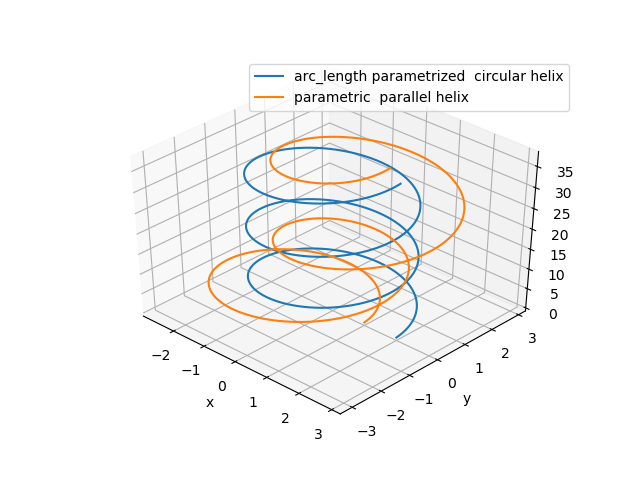
\includegraphics[width=\linewidth, width=12cm, height=10cm]{24_constant=0_1.png}
     \caption{const = 0, the value of $\theta$ at $s=0$}
 \end{figure}
 \begin{figure}[!ht]
     \centering
     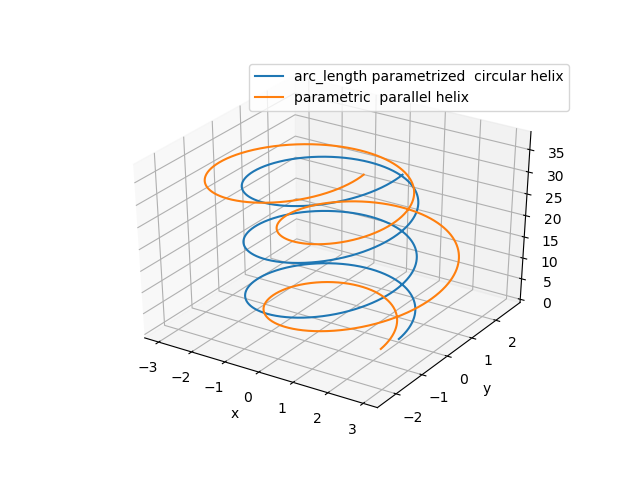
\includegraphics[width=\linewidth, width=12cm, height=10cm]{24_constant=pi2.png}
     \caption{const = $\pi/2$, the value of $\theta$ at $s=0$}
 \end{figure}
.\\
\\
\\
\\
\\
\\


\section*{Problem 25}
\begin{problem}
     Suppose $\alpha$ is an arclength-parametrized curve, P = $\alpha(0)$, and $\kappa(0) \neq 0$. Use Proposition 2.6 to
     establish the following:
     \begin{enumerate}[(\itshape a\normalfont)]
          \item Let Q = $\alpha(s)$ and R = $\alpha(t)$ /. Show that the plane spanned by P, Q, and R approaches the
          osculating plane of $\alpha$ at P as s, $t->0$.
          \item The osculating circle at P is the limiting position of the circle passing through P, Q, and R as
          $s$,$t -> 0$. Prove that the osculating circle has center Z = P + ($1/\kappa(0)$)N(0) and radius $1/\kappa(o)$
          \item The osculating sphere at P is the limiting position of the sphere through P and three neighboring
          points on the curve, as the latter points tend to P independently. Prove that the osculating sphere
          has center\\
          \begin{center}
              $ Z = P + (1/\kappa(0))N(0) + (1/\tau(0)(1/\kappa)^{'}(0))B(0)$
          \end{center}
          and radius
          \begin{center}
               $ \sqrt{(1/\kappa(0))^{2} + (1/\tau(0)(1/\kappa)^{'}(0))^2} $
           \end{center}
          \item How is the result of part c related to Exercise 19?
     \end{enumerate}
\end{problem}
\subsection*{Answer}
\begin{enumerate}[(\itshape a\normalfont)]
     \item In this part, we can prove that the normal of the plane cross through P, Q and R converge the vector is parallel with B(0) which is normal vector of osculating plane
      . We know that the normal of the plane crossing through P,Q and R is $(Q-P) \times (R-P)$. So we have :
      \begin{align}
          (Q-P) & = ((s)-\frac{\kappa_{0}(s)^{3}}{6}) T(0) + (\kappa_{0}/2(s)^{2}+\frac{\kappa^{'}_{0}(s)^{3}}{6}) N(0) + (\frac{\kappa_{0}\tau_{p}(s)^{3}}{6}) B(0) \\
          (R-P) & = ((t)-\frac{\kappa_{0}(t)^{3}}{6}) T(0) + (\kappa_{0}/2(t)^{2}+\frac{\kappa^{'}_{0}(t)^{3}}{6}) N(0) + (\frac{\kappa_{0}\tau_{p}(t)^{3}}{6}) B(0)
     \end{align}
     If we compute $(Q-P) \times (R-P)$, we have:
     \begin{align}
          (Q-P) \times (R-P) & = (\kappa_{0}st(t-s)/2 B(0) + O(s^{3}) or O(t^{3}) \\
     \end{align}
     According to the last equation all terms converge fast to 0 when s,t approaches 0 and just the term of B(0) have large value than other terms. This term is parallel  with B(0).
     \item If we consider C as center of the circle cross the P Q R. we can say that the following function.
     \begin{equation}
           ||\alpha(s)-C||^2  
     \end{equation}
     at least have tree  same values. So its first derivation has at least 2 root and its second derivation has one root at  least. This feature remain as s,t approaches to 0 and the circle converge the osculating circle. So we can write for C as center of osculating circle.
     \begin{align}
          \inner{T_{alpha}(0)}{\alpha(0)-C} & = 0 \\ 
          \inner{T_{alpha}(0)}{T_alpha(0)} + \inner{T_{alpha}^{'}(0)}{\alpha(0)-C} & = 0
    \end{align}
    And we know that the center of the osculating circle is in the osculating plane. So we have :
    \begin{equation}
         C = \alpha(0) + c_{1} T(0) + c_{2} N(0)    
     \end{equation}
     So If we put  C in the equation 3 and 4 , we can compute $c_{1}$ and $c_[2]$. we have:
     \begin{equation}
          c_{1} = 0 ,c_{2} = 1/\kappa(0)     
     \end{equation}
     \item In the same way as previous part, we consider C as center of sphere  crossing through P and three neighborhood. We can say the following function:
     \begin{equation}
          ||\alpha(s)-C||^2  
     \end{equation}
     have at least 4 same value. In the same way as previous part we have: 
     \begin{align}
          \inner{T_{alpha}(0)}{\alpha(0)-C} & = 0 \\ 
          \inner{T_{alpha}(0)}{T_alpha(0)} + \inner{T_{alpha}^{'}(0)}{\alpha(0)-C} & = 0 \\
          \inner{T_{alpha}^{''}(0)}{\alpha(0)-C} & = 0
     \end{align} 
     If we write $ C = \alpha(0) + r_1 N(0) + r_2 T(0) + r_3 B(0)$ and put c in the above equations we have :
     \begin{equation}
          r_{2} = 0 ,r_{1} = 1/\kappa(0) , r_3 = (1/\tau(0)(1/\kappa(0))^{'})  
     \end{equation}
     \item 
     If $\alpha$ lies on a sphere. So the center of osculating sphere at each $\alpha(s)$ is constant and is the center of the sphere
     $\alpha$ lies on it. So we have :
     \begin{equation}
          C = \alpha(s) + (1/\kappa(s)) N(s) +  (1/\tau(s)(1/\kappa(s))^{'}) B(s) 
     \end{equation}
     C is constant If we derivative the above equation we have :
     \begin{equation}
         T(s) + (1/(\kappa(s)))^{'} N(s) + 1/(\kappa(s)) N^{'}(s) +   (1/\tau(s)(1/\kappa(s))^{'})^{'} B(s) +  (1/\tau(s)(1/\kappa(s))^{'}) B^{'}(s) = 0
     \end{equation}  
     If we replace $N^{'}(s)$ with $-\kappa T(s) + \tau B(s)$ and $B^{'}(s)$ with $-\tau(s) N(s)$, we reach the  following equation:
     \begin{equation}
          (\tau(s) / \kappa(s)) + (1/\tau(s)(1/\kappa(s))^{'})^{'} B(s) = 0
     \end{equation}
     which means :
     \begin{equation}
          (\tau(s) / \kappa(s)) + (1/\tau(s)(1/\kappa(s))^{'})^{'} = 0
     \end{equation}
     This is the equation we should prove in Exercise 19 for curve $\alpha$ lying on sphere. we can say :
\end{enumerate}



\section*{Problem 26}
\begin{problem}
     \begin{enumerate}[(\itshape a\normalfont)]
          \item Suppose $\beta$ is a plane curve and $C_{s}$ is the circle centered at $\beta(s)$ with radius r(s). Assuming $\beta$ and
          $r$ are differentiable functions, show that the circle $C_{s}$ is contained inside the circle $C_{t}$ whenever
          $t > s$ if and only if $||\beta^{'}(s)||$ <= $r^{'}(s)$ for all s.
          \item Let $\alpha$be arclength-parametrized plane curve and suppose is a decreasing function. Prove that the
          osculating circle at $\alpha(s)$ lies inside the osculating circle at $\alpha(t)$ whenever $t > s$. (See Exercise 25
          for the definition of the osculating circle.)
     \end{enumerate}
\end{problem}
\subsection*{Answer}
\begin{enumerate}[(\itshape a\normalfont)]
     \item$(\implies) \forall t,\Delta t > 0: ||\beta(t + \Delta t) - \beta(t)|| + r(t) \leqslant r(t + \Delta t)\\  \\ \implies||\frac{\beta(t + \Delta t) - \beta(t)}{\Delta}||\leqslant||\frac{r(t + \Delta t) -r(t)}{\Delta}|| \implies lim||\frac{\beta(t + \Delta t) - \beta(t)}{\Delta}||\leqslant lim||\frac{r(t + \Delta t) -r(t)}{\Delta}||\\  \\ \implies||\beta'(t)||\leqslant r'(t)\\  \\$
     $(\Longleftarrow)\forall t: ||\beta'(t)|| \leqslant r'(t)\\  \\ \implies (u = t+\Delta t)\forall t,\Delta t > 0 : \int_t^u ||\beta'(t)||dt \leqslant r(t +\Delta t) - r(t)\\  \\ \implies  ||\beta(t + \Delta t) - \beta(t)|| + r(t) \leqslant r(t + \Delta t)$
     \item $\beta(s) = \alpha(s) + \frac{N(S)}{k(s)} , r(s) = \frac{1}{k}\\  \\ \implies \beta'(s) = \alpha'(s) + \frac{-k^(2)\alpha' - k'N}{k^2} = \frac{-k'(s)}{k^2(s)}N(s)\\  \\ \implies ||\beta'(s)|| = \frac{-k'(s)}{k^2(s)} \leqslant r'(s)\\  \\ \implies \forall t > s:\\  \\ ||\beta(t) - \beta(s)|| + r(s) \leqslant r(t)$
\end{enumerate}

\section*{Problem 27}
\begin{problem}
     Suppose the front wheel of a bicycle follows the arclength-parametrized plane curve $\alpha$. Determine the
     path $\beta$ of the rear wheel, 1 unit away, as shown in Figure 2.8. (Hint: If the front wheel is turned an
     angle $\theta$ from the axle of the bike, start by writing $\alpha - \beta$ in terms of $\theta$ , T, and N. Your goal should be
     a differential equation that $\theta$ must satisfy, involving only $\kappa$ . Note that the path of the rear wheel will
     obviously depend on the initial condition $\theta(0)$. In all but the simplest of cases, it may be impossible to
     solve the differential equation explicitly.)
\end{problem}
\begin{figure}[htbp]
     \centering
     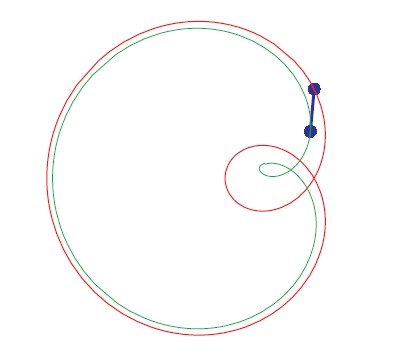
\includegraphics[width=\linewidth, width=12cm, height=11cm]{question_27.jpg}
     \caption{<caption>}
     \label{<label>}
\end{figure}
\subsection*{Answer}
Assumptions are:
\begin{enumerate}
     \item $||\alpha - \beta|| = 1$
     \item $||\alpha'|| = 1$
     \item $||\frac{\alpha''}{k}|| = 1$
     \item $\alpha'\bot\alpha''$
\end{enumerate}
So we have
\begin{align*}
     &\implies	\alpha - \beta = \cos(\theta)\alpha' + \frac{\sin(\theta)}{k}\alpha'' \implies\beta = \alpha - \cos(\theta)\alpha' - \frac{\sin(\theta)}{k}\alpha''\\
     &\implies \beta' =\alpha' + \sin(\theta)\theta'\alpha' - \cos(\theta)\alpha'' - \frac{\cos(\theta)\theta'\alpha''}{k\alpha} + \sin(\theta)k\alpha'\\
     &\implies \beta' =\alpha'(1 + \sin(\theta)\theta' + k\sin(\theta)) - \alpha''(\cos(\theta) + \frac{\cos(\theta)\theta'}{k})\\
\end{align*}
Note that bicycle constraint is that $\beta' \parallel \alpha - \beta$ so :
\begin{align*}
     &\implies-\cos(\theta)^2 ( 1 + \frac{\theta'}{k}) = \frac{\sin(\theta)}{k}(1 + \sin(\theta)\theta' + k\sin(\theta))\\
     &\implies\frac{\sin(\theta)}{k} + \frac{\sin(\theta)^(2)\theta'}{k} + \sin(\theta)^2 + \cos(\theta)^2 + \frac{\cos(\theta)^(2)\theta'}{k} = 0\\
     &\implies\frac{\theta'}{k} + 1 + \frac{\sin(\theta)}{k} = 0\\
     &\implies\theta' + \sin(\theta) + k = 0\\
\end{align*}
\end{document}




